\chapter{Representation of vortex variability in climate models}
\label{cha:models}




\begin{table}[h]
\small
\centering
\begin{tabular}{lcccccc} \hline
Model          & Ensemble size & Lid/ km & Levels & dh/km & d$z_{1}$/km & d$z_{2}$/km \\ \hline
CanESM2        & 5 & 48.1    & 35     & 268          & 1.48         & 2.30          \\
CMCC-CESM      & 1 & 80.6    & 39     & 536          & 1.49         & 1.89          \\
CMCC-CMS       & 1 & 80.6    & 95     & 268          & 0.65         & 0.68          \\
GFDL-CM3       & 5 & 76.3    & 48     & 191          & 1.32         & 1.75           \\
HadGEM2-CC     & 3 & 84.1    & 60     & 144          & 0.82         & 1.18          \\
IPSL-CM5A-LR   & 5 & 70.4    & 39     & 254          & 1.21         & 1.75          \\
IPSL-CM5A-MR   & 3 & 70.4    & 39     & 169          & 1.21         & 1.75          \\
IPSL-CM5B-LR   & 1 & 70.4    & 39     & 254          & 1.21         & 1.75          \\
MIROC-ESM-CHEM & 1 & 87.8    & 80     & 399          & 0.77         & 0.73          \\
MPI-ESM-LR     & 3 & 80.6    & 47     & 268          & 0.87         & 1.70            \\
MPI-ESM-MR     & 3 & 80.6    & 95     & 268          & 0.65         & 0.68          \\
MRI-CGCM3      & 1 & 80.6    & 48     & 107          & 0.88         & 1.87          \\
MRI-ESM1       & 1 & 80.6    & 48     & 107          & 0.88         & 1.87 \\ \hline 
\end{tabular}
\caption[CMIP5 model parameters.]{Parameters of the CMIP5 models studied in this
  chapter. Where the model lid is defined in terms of a pressure, its height was
  estimated using $z=-H\mathrm{log}(p/p_{0})$ with $H=7$~km and
  $p_{0}=1000$~hPa. Horizontal resolution, d$h$, is estimated at 45$^{\circ}$N
  and vertical resolution is shown averaged over two regions; 5-15~km (d$z_{1}$)
  and 15-30~km (d$z_{2}$).} 
\end{table}







\begin{figure}
 \centering
 \noindent\includegraphics[width=\textwidth]{figures/chapter-models/moments_stats1.pdf}
 \caption[Distributions of moment diagnostics for the CMIP5
 models.]{Distributions of centroid latitude and aspect ratio for the ERA (grey
   lines) (a) and the CMIP5 models (red lines). Joint distributions are shown
   with a logarithmic scale such that red squares represent the densest
   regions.}
 \label{Fig2}
\end{figure}

\begin{figure}
 \ContinuedFloat
 \centering
 \noindent\includegraphics[width=\textwidth]{figures/chapter-models/moments_stats2.pdf}
 \caption[]{(Continued)}
 \label{Fig2}
\end{figure}
 
\begin{figure}
 \centering
 \noindent\includegraphics[width=\textwidth]{figures/chapter-models/moments_seasonal_stats.pdf}
 \caption[Seasonal cycle of moment diagnostics in the CMIP5 models]{Seasonal
   cycle of aspect ratio and centroid latitude in ERA (black) and the CMIP5
   models (colours). Thick lines represent the mean and thin lines the 95th or
   5th percentile for aspect ratio and centroid latitude respectively.}
 \label{Fig2}
\end{figure}



\begin{figure}
 \centering
 \noindent\includegraphics[width=\textwidth]{figures/chapter-models/events_seasonal.pdf}
 \caption[Seasonal distribution of splits and displacements in the CMIP5
 models]{Seasonal distribution of the occurrence of split and displaced vortex
   events in ERA (a) and the CMIP5 models.}
 \label{Fig2}
\end{figure}

\begin{figure}
 \centering
 \noindent\includegraphics[width=\textwidth]{figures/chapter-models/events_bar_stacked.pdf}
 \caption[Frequency of split and displaced vortex events in the CMIP5
 models]{Frequency of split and displaced vortex events in the CMIP5
   models. Error bars are for the frequency of all events, and represent one
   $\sigma$ range, assuming a binomial distribution of events. The grey shaded
   region represents the one $\sigma$ range for ERA, along with the mean (dashed
   line.) }
 \label{Fig2}
\end{figure}

\begin{figure}
 \centering
 \noindent\includegraphics[width=\textwidth]{figures/chapter-models/10hPa_GPH_composites.pdf}
 \caption[Composites of 10~hPa $Z$ at the onset date split and displaced vortex
 events in the CMIP5 models.]{Composites of 10~hPa $Z$ at the onset date of
   split (S) and displaced (D) vortex events in ERA (a,b) and the CMIP5
   models. The number of events entering the composite and their type are
   shown in the title of each plot. The contour interval is 0.3~km.}
 \label{Fig2}
\end{figure}

\begin{figure}
 \centering
 \noindent\includegraphics[width=\textwidth]{figures/chapter-models/CMIP5_moments_scatter.pdf}
 \caption[Comparison of moment diagnostics and frequency of split and displaced
 vortex events.]{Comparison of the DJFM mean aspect ratio with frequency of
   split vortex events (a) and DJFM mean centroid latitude with frequency of
   displaced vortex events (b) in the CMIP5 ensemble and ERA. A linear best fit
   and the correlation coefficients for all the models are also shown.}
 \label{Fig2}
\end{figure}




\begin{figure}
 \centering
 \noindent\includegraphics[width=\textwidth]{figures/chapter-models/dripping_paint1.pdf}
 \caption[NAM composites for splits and displacements in the CMIP5
 models]{Composites of normalised polar cap averaged $Z$ anomalies following
   split and displaced vortex events in ERA (a,b), the CMIP5 models, and the
   multi-model mean (C,D). Numbers in the upper right of each plot represent the
   number of events entering the composite.}
 \label{Fig2}
\end{figure}

\begin{figure}
 \ContinuedFloat
 \centering
 \noindent\includegraphics[width=\textwidth]{figures/chapter-models/dripping_paint2.pdf}
 \caption[]{(Continued)}
 \label{Fig2}
\end{figure}

\begin{figure}
 \centering
 \noindent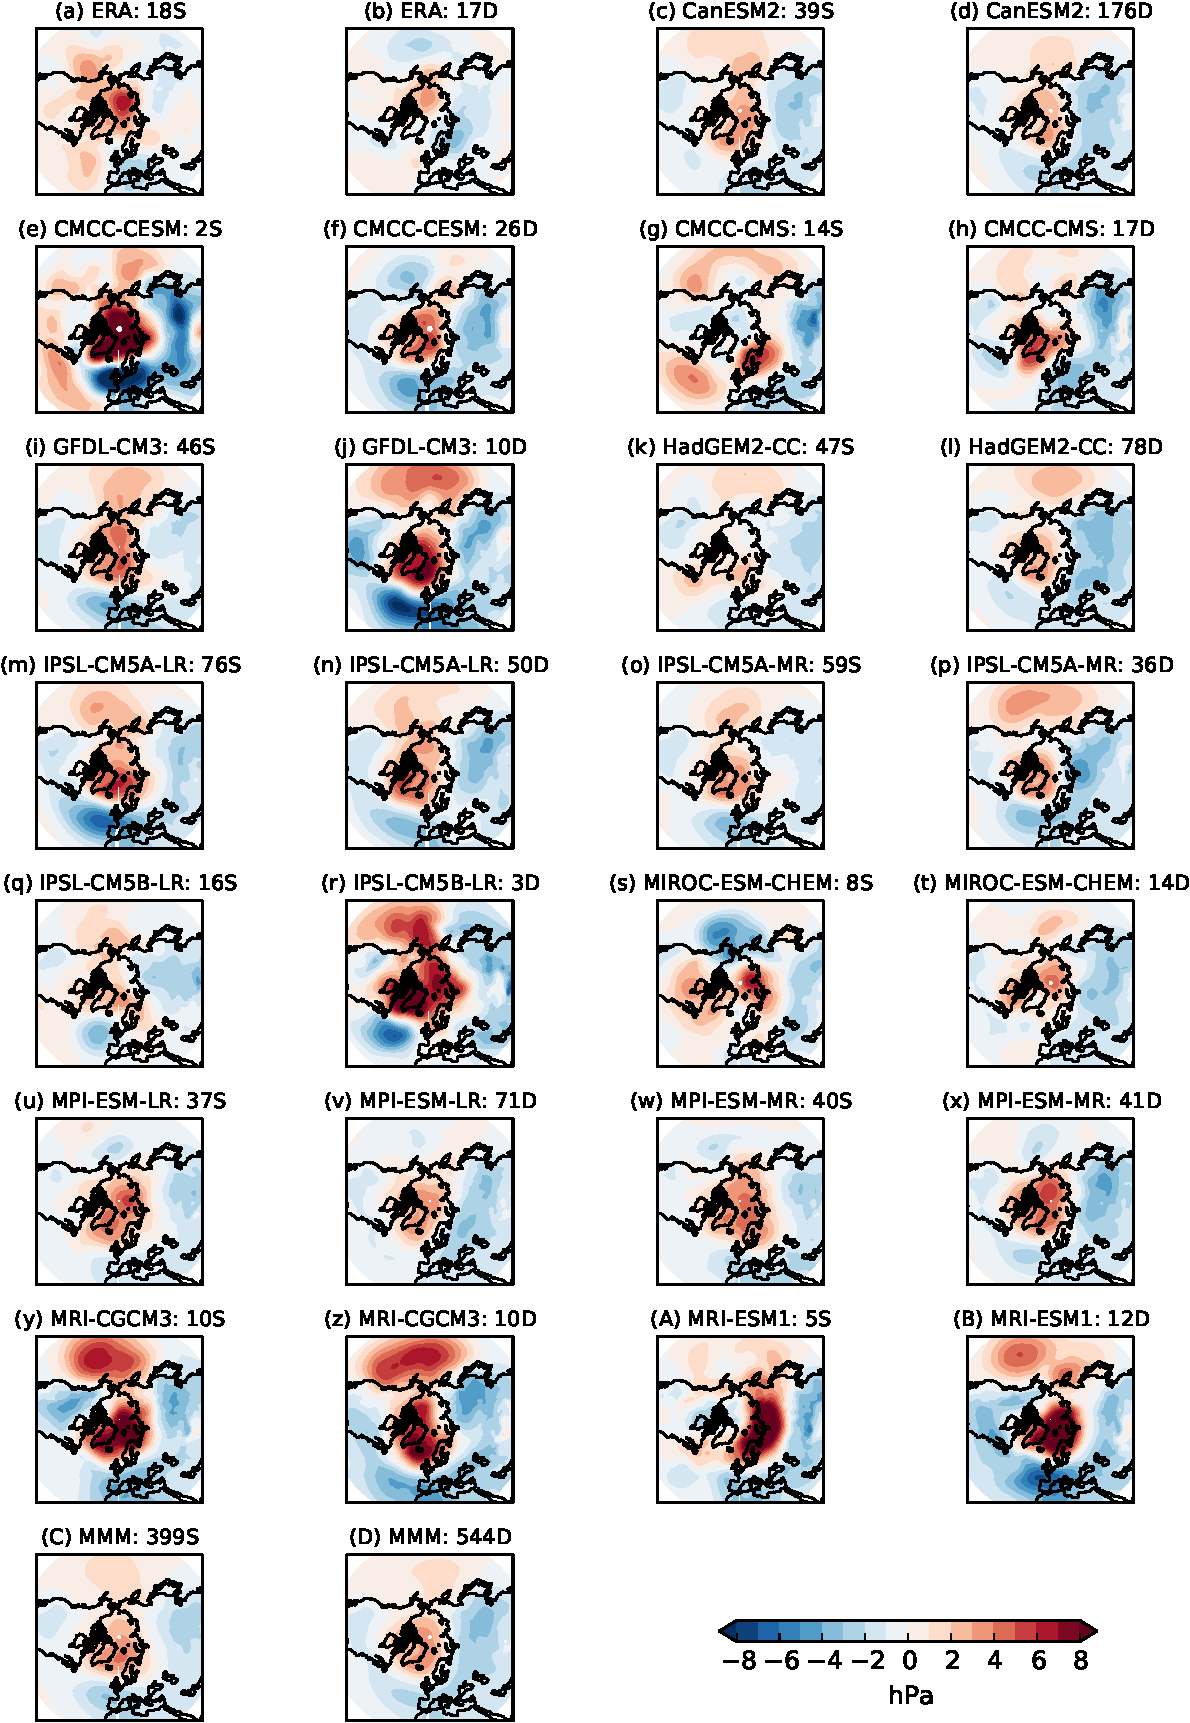
\includegraphics[width=\textwidth]{figures/chapter-models/mslp_composites.pdf}
 \caption[MSLP composites following splits and displacements in the CMIP5
 models]{Composites of mean sea-level pressure averaged 0-30 days following
   split (S) and displaced (D) vortex events in the CMIP5 ensemble. Also shown
   are the ERA composite (a,b) and the multi-model mean (C,D). The multi-model
   mean is calculated as to give each event an equal weighting.}
 \label{Fig2}
\end{figure}

\begin{figure}
 \centering
 \noindent\includegraphics[width=\textwidth]{figures/chapter-models/mslp_diff.png}
 \caption[Difference of MSLP following split and displaced vortex
 events.]{Difference (S-D) of composites of mean sea-level pressure averaged 0-30 days
   following split (S) and displaced (D) vortex events in ERA and the CMIP5
   ensemble. Stippling indicates regions that are $>$95\% significant according
   to a two-tailed bootstrap test.}
 \label{Fig2}
\end{figure}


\begin{figure}
 \centering
 \noindent\includegraphics[width=\textwidth]{figures/chapter-models/scatter_matrix.pdf}
 \caption[Relationship between model resolution and split and displaced vortex
 events in the CMIP5 models.]{Relationship between model resolution and
   representation of split and displaced vortex events in the CMIP5
   models. Model resolution is shown as horizontal resolution ($\mathrm{d}h$),
   vertical resolution ($\mathrm{d}z$) over 5-15~km and 15-30~km, and aspect
   ratio ($\mathrm{d}z$(5-15~km)$ / \mathrm{d}h$. Also shown is the number of
   SSWs per decade, the fraction of SSWs that are splits, and the average NAM at
   500~hPa 0-30 days following SSWs. Histograms for the relevant quantities
   are shown along the leading diagonal.}
 \label{Fig2}
\end{figure}

%%% Local Variables:
%%% mode: latex
%%% TeX-master: "thesis"
%%% End:
